\documentclass[a4paper,11pt,oneside]{article}
\usepackage[pdftex]{graphicx}
\usepackage[utf8]{inputenc}
\usepackage[spanish]{babel}
\usepackage{fancyhdr}
\usepackage[usenames,dvipsnames]{color}
\usepackage{colortbl}
\usepackage{tabularx}
\usepackage{hyperref}
\usepackage{pdfpages}
\usepackage{lscape}


\setlength{\headheight}{15.2pt}
\pagestyle{fancy}

\lhead{\nouppercase{\leftmark}}
\chead{}
\rhead{}

\hypersetup{
colorlinks,
citecolor=black,
filecolor=black,
linkcolor=black,
urlcolor=black
}

\setlength{\parskip}{6pt}

\begin{document}

%%%% Title Page %%%%%

%\pagenumbering{alph}

\begin{titlepage}
\begin{center}

% Upper part of the page

\includegraphics[width=0.2\textwidth]{img/logo-uclm.png}\\[1cm]
\textsc{\LARGE Escuela Superior de Informática}\\[0.5cm]
\textsc{\Large Universidad de Castilla -- La Mancha}\\[2.5cm]

% Title
{\LARGE Práctica 1}\\[0.5cm]
\rule{\linewidth}{0.5mm}\\[0.4cm]
{\huge \textbf{Tres en Raya Definitivo}}\\
\rule{\linewidth}{0.5mm}\\[0.4cm]

% Authors
\begin{minipage}{0.5\textwidth}
\begin{flushleft}
\large
\hspace{1cm}\textbf{\emph{Autores}}\\
Marchán Loro, Javier\\
Peralta López, Ángel\\
Pérez Pascual, Rubén\\
Ruedas García, Antonio\\
\end{flushleft}
\end{minipage}
\vfill

% Bottom of the page
\begin{minipage}{\textwidth}
\large
\begin{tabular}{rl}
\textbf{Asignatura}: & Ingeniería del Software II\\
\textbf{Titulación}: & Ingeniería Informática\\
\textbf{Fecha}: & \today
\end{tabular}
\end{minipage}

\end{center}
\end{titlepage}

%%%% end Title Page %%%%%

\pagenumbering{roman}
\setcounter{page}{1}

\tableofcontents
\clearpage

\pagenumbering{arabic}
\setcounter{page}{1}

\clearpage
\section{Introducción}

Este documento describe el análisis, desarrollo e implementación llevados a cabo para obtener
el juego \textbf{Tres en Raya Definitivo} \footnote{Este documento no explica las reglas del juego}.

Se trata de una aplicación cliente-servidor para escritorio que se comunica a través de RMI.
El lenguaje utilizado para la implementación ha sido Java.

Este documento pretende que el lector obtenga una idea clara de la composición del sistema, para ello
se ha dividido en distintas secciones. En primer lugar los requisitos funcionales ayudan a entender el objetivo
buscado. La arquitectura del sistema junto con los casos de uso son las secciones más importantes, ya
que ayudarán al lector a hacerse una imagen mental, a alto nivel, del sistema desarrollado.

El resto de secciones profundizan en el conocimiento del sistema.

\clearpage

\section{Requisitos funcionales}

\subsection{Registrarse}

{\footnotesize
\begin{tabularx}{0.95\textwidth}{p{0.2\textwidth}|X}

\textbf{Caso de uso} & \textbf{Registrarse} \\
& \\
\textbf{Precondición} & No está registrado \\

\textbf{Escenario general} & \begin{enumerate}
\item El usuario pulsa el botón de registrarse en la ventana de inicio.
\item Se muestra la ventana de registro.
\item El usuario introduce su email y su contraseña en la ventana de registro.
\item El usuario pulsa el botón de confirmación.
\item Se espera confirmación por parte del servidor.
\item La ventana de inicio informa al usuario del éxito de la operación.
\end{enumerate} \\

\textbf{Poscondición} & Un nuevo usuario existe en el sistema.\\
& \\
& \\
\textbf{Precondición} & Ya está registrado\\
\textbf{Escenario alternativo} & \begin{enumerate}
 \item El usuario pulsa el botón de registrarse en la ventana de inicio.
\item Se muestra la ventana de registro.
\item El usuario introduce su email y contraseña en la ventana de registro.
\item El usuario pulsa el botón de confirmación.
\item Se espera confirmación por parte del servidor.
\item La ventana de inicio informa al usuario que ya se encuenta registrado.
\end{enumerate}\\
\textbf{Poscondición}& No se registra el usuario de nuevo.\\

\end{tabularx}
}

\subsection{Iniciar sesión}

{\footnotesize
\begin{tabularx}{0.95\textwidth}{p{0.2\textwidth}|X}

\textbf{Caso de uso} & \textbf{Iniciar sesión} \\
& \\
\textbf{Precondición} & Usuario registrado y aún no logeado \\

\textbf{Escenario general} & \begin{enumerate}
\item El usuario introduce su email y contraseña en la ventana de inicio.
\item El usuario pulsa el botón de ``Iniciar sesión''.
\item Se espera validación por parte del servidor.
\item Se cierra la ventana de login y se abre la lista de jugadores.
\end{enumerate} \\

\textbf{Poscondición} & Se ejecuta el caso de uso ``Ver lista de jugadores''
\\
& \\
& \\
\textbf{Precondición} & Datos de acceso incorrectos\\
\textbf{Escenario alternativo} & \begin{enumerate}
\item El usuario introduce su email y contraseña en la ventana de inicio.
\item El usuario pulsa el botón de ``Iniciar sesión''.
\item Se espera validación por parte del servidor.
\item Se informa al usuario que los datos de acceso son incorrectos.
\end{enumerate}\\
\textbf{Poscondición} &Usuario no logeado.\\
& \\
& \\
\textbf{Precondición} & Usuario ya logeado.\\
\textbf{Escenario alternativo}& \begin {enumerate}
\item El usuario introduce su email y contraseña en la ventana de inicio.
\item El usuario pulsa el botón de ``Iniciar sesión''.
\item Se espera validación por parte del servidor.
\item Se informa al usuario que ya está logeado.
\end{enumerate}\\
\textbf{Poscondición}& Usuario no logeado de nuevo.\\
\end{tabularx}
}

\subsection{Cerrar sesión}

{\footnotesize
\begin{tabularx}{0.95\textwidth}{p{0.2\textwidth}|X}

\textbf{Caso de uso} & \textbf{Cerrar sesión} \\
& \\
\textbf{Precondición} & Sesión iniciada \\

\textbf{Escenario general} & \begin{enumerate}
\item El usuario pulsa el botón de cerrar el programa.
\item Se manda una petición de cierre de sesión al servidor.
\item El servidor cierra la sesión del usuario.
\item Se cierra el programa.
\end{enumerate} \\

\textbf{Poscondición} & El usuario deja de estar activo en el servidor y deja de aparecer
en la lista de jugadores.\\

& \\
& \\
\textbf{Precondición} & Sesión iniciada y jugador en partida \\

\textbf{Escenario alternativo} & \begin{enumerate}
\item El usuario pulsa el botón de cerrar el programa.
\item Se manda una petición de cierre de sesión al servidor.
\item El servidor elimina la partida y cierra la sesión del usuario.
\item Se cierra el programa.
\end{enumerate} \\

\textbf{Poscondición} & El usuario deja de estar activo en el servidor y deja de aparecer
en la lista de jugadores.

\end{tabularx}
}

\subsection{Salir de la partida}
{\footnotesize
\begin{tabularx}{0.95\textwidth}{p{0.2\textwidth}|X}

\textbf{Caso de uso} &\textbf{Salir de la partida} \\
& \\
\textbf{Precondición} & Estar conectado a una partida.\\

\textbf{Escenario general} & \begin{enumerate}
\item El usuario pulsa el botón cerrar partida en la ventana de juego.
\item Se comunica al servidor que elimmine la partida.
\item Se cierra la ventana de juego.

\end{enumerate} \\

\textbf{Poscondición} & Se sale de la partida y aparece la ventana principal.

\end{tabularx}
}

\subsection{Retar jugador}
{\footnotesize
\begin{tabularx}{0.95\textwidth}{p{0.2\textwidth}|X}

\textbf{Caso de uso} & \textbf{Retar jugador} \\
& \\
\textbf{Precondición} & Sesión iniciada y oponente en el sistema \\

\textbf{Escenario general} & \begin{enumerate}
\item El usuario selecciona un jugador de la lista y pulsa ``Retar''.
\item Se manda la petición al servidor que a su vez se lo comunica al oponente.
\item El servidor busca al oponente y le envia la solicitud de reto.
\end{enumerate} \\

\textbf{Poscondición} & Usuario espera confirmación del oponente.

\end{tabularx}
}

\subsection{Aceptar reto}
{\footnotesize
\begin{tabularx}{0.95\textwidth}{p{0.2\textwidth}|X}

\textbf{Caso de uso} & \textbf{Aceptar reto} \\
& \\
\textbf{Precondición} & Sesión iniciada y petición de reto realizada\\

\textbf{Escenario general} & \begin{enumerate}
\item Se abre ventana emergente de invitación a partida.
\item El usuario pulsa el botón de aceptar.
\item Se notifica al servidor de la aceptación.
\end{enumerate} \\

\textbf{Poscondición} & Se crea una partida.\\
& \\
& \\
\textbf{Precondición} & Sesión iniciada y petición de reto realizada\\
\textbf{Escenario alternativo} & \begin{enumerate}
\item Se abre ventana emergente de invitación a partida.
\item El usuario pulsa el botón de cancelar.
\item Se notifica al servidor de la cancelación.
\end{enumerate}\\

\textbf{Poscondición}& No se crea partida y se vuelve a la GUI de la lista de jugadores.

\end{tabularx}
}

\subsection{Realizar movimiento}
{\footnotesize
\begin{tabularx}{0.95\textwidth}{p{0.2\textwidth}|X}

\textbf{Caso de uso} & \textbf {Realizar movimiento válido} \\
& \\
\textbf{Precondición} & Existencia de una partida \\

\textbf{Escenario general} & \begin{enumerate}
\item El usuario coloca una pieza en el tablero de juego.
\item Se comprueba la validez del movimiento.
\item Se manda información del movimiento al servidor.

\end{enumerate} \\

\textbf{Poscondición} & Tablero modificado.\\
& \\
& \\
\textbf{Precondición} & Realizar movimiento no válido\\
\textbf{Escenario alternativo} & \begin{enumerate}
\item El usuario coloca una pieza en el tablero de juego.
\item Se comprueba la validez del movimiento.
\item Se informa al usuario de que el movimiento no es válido.

\end{enumerate} \\

\textbf{Poscondición} & Tablero no modificado.

\end{tabularx}
}

\subsection{Ver la lista de jugadores}

{\footnotesize
\begin{tabularx}{0.95\textwidth}{p{0.2\textwidth}|X}

\textbf{Caso de uso} & \textbf{Ver la lista de jugadores} \\
& \\
\textbf{Precondición} & Iniciar sesión \\

\textbf{Escenario general} & \begin{enumerate}
\item Se abre la ventana de la lista de jugadores y recibe la lista de
usuarios conectados del servidor.

\end{enumerate} \\

\textbf{Poscondición} & La lista de jugadores está disponible para el usuario.\\
 & \\
& \\
\textbf{Precondición} & Jugador ya iniciado sesión y otro jugador se conecta.\\
\textbf{Escenario alternativo} & \begin{enumerate}
\item El servidor envía al usuario la lista de jugadores actualizada.
\end{enumerate}\\
\textbf{Poscondición}& Ambos jugadores con la lista de jugadores actualizada.\\
\end{tabularx}
}


\subsection{Enviar Petición de Reto}

{\footnotesize
\begin{tabularx}{0.95\textwidth}{p{0.2\textwidth}|X}

\textbf{Caso de uso} & \textbf{Enviar petición de Reto}\\
& \\
\textbf{Precondición} & Usuarios logeados en el sistea y petición de reto realizada. \\

\textbf{Escenario general} & \begin{enumerate}

\item Al servidor le llega una petición de reto por parte de un usuario.
\item El servidor envía al otro jugador la petición de reto.

\end{enumerate} \\

\textbf{Poscondición} &  \\ \\

\end{tabularx}
}

\subsection{Registrar un movimiento}

{\footnotesize
\begin{tabularx}{0.95\textwidth}{p{0.2\textwidth}|X}

\textbf{Caso de uso} & \textbf{Registrar un movimiento} \\
& \\
\textbf{Precondición} & Iniciar sesión, Unirse a una partida y Conectarse a una
partida \\

\textbf{Escenario general} & \begin{enumerate}
\item Al servidor le llega el movimiento realizado por un usuario.
\item El servidor almacena el movimiento en la base de datos.
\item El servidor notifica al otro usuario que ya puede realizar su movimiento.
\end{enumerate} \\

\textbf{Poscondición} & Se realiza el caso de uso: ''Enviar actualización de la
partida''.\\

\end{tabularx}
}

\subsection{Responder a solicitud de reto}
{\footnotesize
\begin{tabularx}{0.95\textwidth}{p{0.2\textwidth}|X}

\textbf{Caso de uso} & \textbf{Responder a solicitud de reto} \\
& \\
\textbf{Precondición} & Iniciar sesión\\

\textbf{Escenario general} & \begin{enumerate}
\item El servidor envía al usuario la solicitud de reto del otro usuario.
\item El cliente recibe la solicitud y la envía al controlador.
\item El controlador la envía a la ventana de jugadores para que muestre que el jugador ha sido retado
\item El usuario elige la acción en la ventana (si acepta o si no).
\item La ventana de juego envía la información al controlador.
\item La fachada envía la respuesta al servidor por medio del proxy.
\end{enumerate} \\

\textbf{Poscondición} & Respuesta a reto enviada.

\end{tabularx}
}

\subsection{Realizar movimiento}

{\footnotesize
\begin{tabularx}{0.95\textwidth}{p{0.2\textwidth}|X}

\textbf{Caso de uso} & \textbf{Realizar Movimiento} \\
& \\
\textbf{Precondición} & El usuario debe haberse unido a una partida y estar
conectado a ella. \\

\textbf{Escenario general} & \begin{enumerate}
\item El usuario pulsa sobre la casilla del tablero a colocar.
\item La interfaz avisa al controlador del movimiento.
\item El controlador envía el movimiento a la fachada.
\item La fachada envía el movimiento a Tablero9x9.
\item Tablero9x9 comprueba la legalidad del movimiento.
\item Si el movimiento es válido se lo envía al proxy y avisa al controlador para realizar el camino inverso hacia la interfaz y colocar la ficha.
\item Si el movimiento es inválido se lanza una excepción que se recoge en el controlador.
\item El controlador envía la excepción a la interfaz de usuario para comunicarle el error que ha cometido.
\end{enumerate} \\
\textbf{Postcondición} & Movimiento realizado. \\
\end{tabularx}
}



\section{Otros requisitos}
\subsection{Requisitos de la interfaz de usuario}
\subsubsection{Ventana de inicio}
{\footnotesize

 \textbf{Descripción:} Da la bienvenida al usuario.\\ Debe permitir al usuario
ejecutar el
caso de uso ``Iniciar sesión'' e introducir los siguientes datos: \\

\begin{tabularx}{0.9\textwidth}{llX}
\hline
\textbf{Dato} & \textbf{Tipo} & \textbf{Descripción} \\
\hline
NombreUsuario & Texto & Nombre del usuario \\
Contraseña & Texto & Contraseña en el sistema \\
\hline
\end{tabularx}
}

\subsubsection{Ventana de registro}
{\footnotesize



 \textbf{Descripción:} Permite registrarse al usuario.\\
Es necesario que
permita al usuario introducir los siguientes datos: \\

\begin{tabularx}{0.9\textwidth}{llX}
\hline
\textbf{Dato} & \textbf{Tipo} & \textbf{Descripción} \\
\hline
Nombre & Texto & Nombre del usuario \\
eMail & Texto & Dirección de correo electrónico \\
Contraseña & Texto & Contraseña en el sistema \\
Conf. Contraseña & Texto & Confirmación de contraseña \\
\hline
\end{tabularx}

}

\subsubsection{Ventana principal}
{\footnotesize

 \textbf{Descripción:}  Mostrará al usuario las partidas disponibles y las
partidas en
juego.\\
Es necesario que
permita al usuario ejecutar los siguientes casos de uso: \\
\begin{enumerate}
\item Crear una partida.
\item Unirse a una partida.
\item Conectarse a una partida.
\item Ver lista de partidas.

\end{enumerate}
}

\subsubsection{Ventana Crear partida}
{\footnotesize

 \textbf{Descripción:}  Permite al usuario crear una nueva partida.\\
Es necesario que
permita al usuario introducir los siguientes datos: \\

\begin{tabularx}{0.9\textwidth}{llX}
\hline
\textbf{Dato} & \textbf{Tipo} & \textbf{Descripción} \\
\hline
Nombre & Texto & Nombre de la partida \\
Días de juego & Fecha & Días en los que se jugará la partida\\
Hora de Inicio de Juego & Hora & Hora en la que empieza o continua la partida
los días indicados\\
Hora de Fin de Juego & Hora & Hora en la que termina la partida los días
indicados\\
\hline
\end{tabularx}
}

\subsubsection{Ventana de juego}
{\footnotesize



 \textbf{Descripción:}  Muestra al usuario todos los detalles de una partida y
permite
jugar en ella. Deberá mostrar el tablero de juego con la asignación de
territorios.\\

Es necesario que
permita al usuario ejecutar los siguientes casos de uso: \\
\begin{enumerate}
\item Desconectarse de una partida.
\item Realizar un movimiento.
\item Responder acción enemiga.
\item Comprar refuerzos.
\item Enviar petición de alianza.
\item Responder a petición de alianza.
\item Romper alianza.

\end{enumerate}


}

\clearpage

\section{Arquitectura del sistema} 

En la Figura \ref{arq_sistema} se muestra una visión de la arquitectura del sistema. Se
trata de una arquitectura cliente-servidor a través de RMI. El cliente usa
un proxy para comunicarse con el servidor y éste conoce un proxy de cada
cliente con el que se comunica. Toda la logica del juego reside en el cliente.

 \begin{figure}[h]
 \centering
 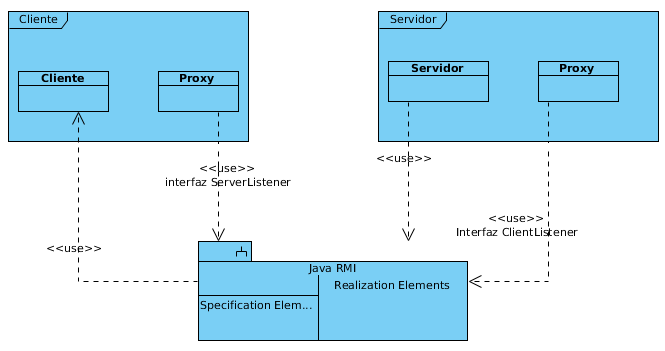
\includegraphics[scale=0.65]{img/arquitectura/arquitectura.png}
 \caption{Arquitectura del sistema}
 \label{arq_sistema}
 \end{figure}

\subsection{Arquitectura del cliente}
 
En la Figura \ref{arq_cliente} se muestra la arquitectura del cliente. Se ha utilizado una arquitectura MVC.
Además, se incluye una capa de comunicación:

\begin{itemize}
 \item \emph{Presentación:} Contiene las clases de las ventanas que se muestran al usuario y las interfaces que implementan.
 \item \emph{Controlador:} Contiene la lógica de control. Se encarga de comunicar a la interfaz los cambios de estado de la
 capa de dominio y de modificar el estado del dominio atendiendo a los cambios en la interfaz del juego.
 \item \emph{Dominio:} Contiene toda la lógica del juego. La clase Tablero9x9 es la clase principal e implementa las reglas del 
 juego. Se utiliza el patrón fachada para obtener un punto de acceso único a la capa de dominio. La clase encargada de 
 esta abstracción es FTERD.
 \item \emph{Comunicación:} Contiene las clases que realizan la función de \emph{listener} como es el caso de la clase Cliente,
 y el proxy con el servidor. Estas clases solamente se encargan del envío de los respectivos mensajes al servidor o a la fachada
 del paquete de dominio.
\end{itemize}

 \begin{figure}[h]
 \centering
 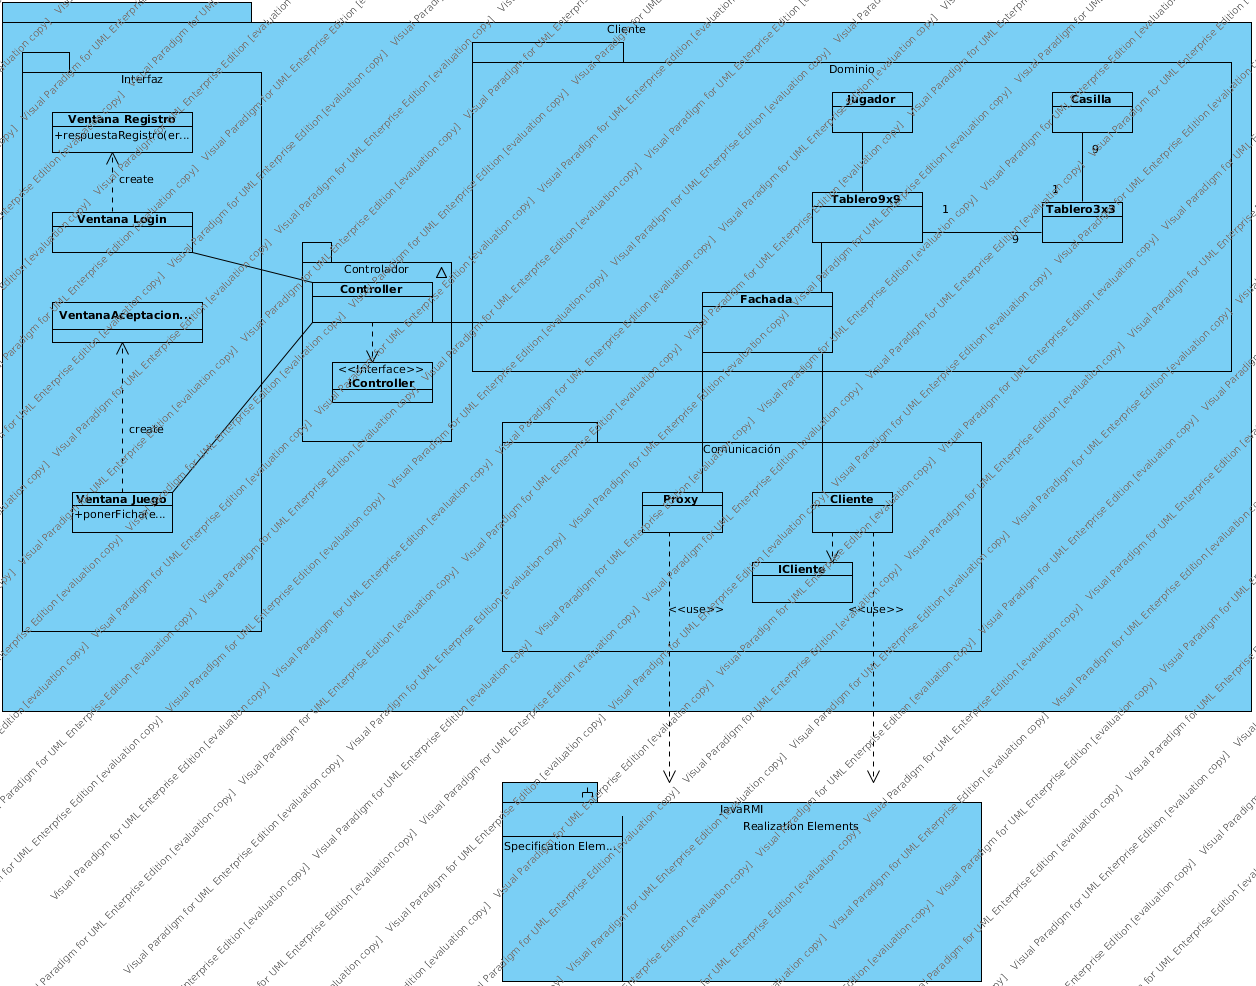
\includegraphics[scale=0.4]{img/arq_Cliente.png}
 \caption{Arquitectura del cliente}
 \label{arq_cliente}
 \end{figure}

\subsection{Arquitectura del servidor}

En la Figura \ref{arq_servidor} se muestra la arquitectura multicapa del servidor:

\begin{itemize}
 \item \emph{Comunicación:} Contiene las clases encargadas de la comunicación, en este caso la clase servidor y su interfaz
 RMI. La clase servidor actúa como \emph{listener} para escuchar solicitudes de los clientes. También responde a esos clientes,
 ya que internamente guarda una hash con los clientes que se han dado de alta en el sistema.
 \item \emph{Persistencia:} Contiene las clases encargadas de almacenar las partidas y sus respectivos tableros, jugadores
 y movimientos. Entre esas clases está la base \emph{Broker}, que actúa como agente entre el subsistema de base de datos y
 el sistema del servidor. Se ha optado por utilizar un patrón de fabricación pura en lugar de seguir el patrón experto para
 la persistencia. De esta forma, un conjunto de clases \emph{DAO} especializadas se encargan de almacenar los diferentes
 aspectos del dominio.
 \item \emph{Dominio:} Contiene las clases de dominio como las encargadas de representar a cualquier juego, además de la
 clase Fachada. Esta clase contiene una referencia a cada uno de los modelos que se están jugando en el sistema, es decir,
 contiene todos los tableros activos.
\end{itemize}


 \begin{figure}[h]
 \centering
 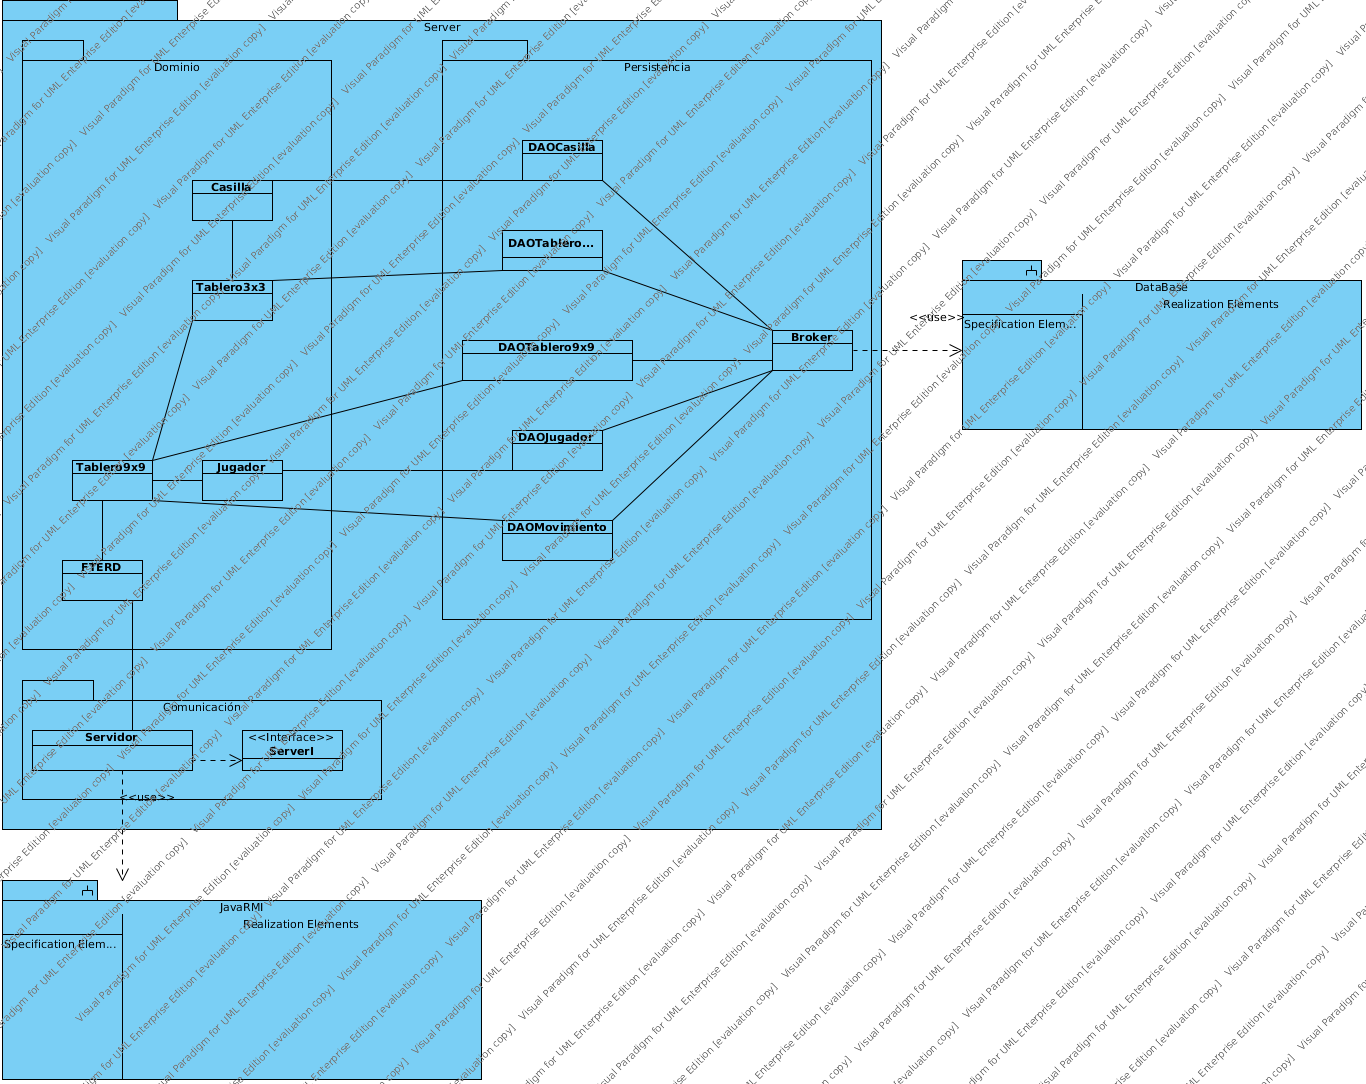
\includegraphics[scale=0.4]{img/arq_Servidor.png}
 \caption{Arquitectura del servidor}
 \label{arq_servidor}
 \end{figure}
 
\clearpage

\section{Casos de uso} 
\subsection{Diagrama de casos de uso del cliente}
 \begin{figure}[h]
 \centering
 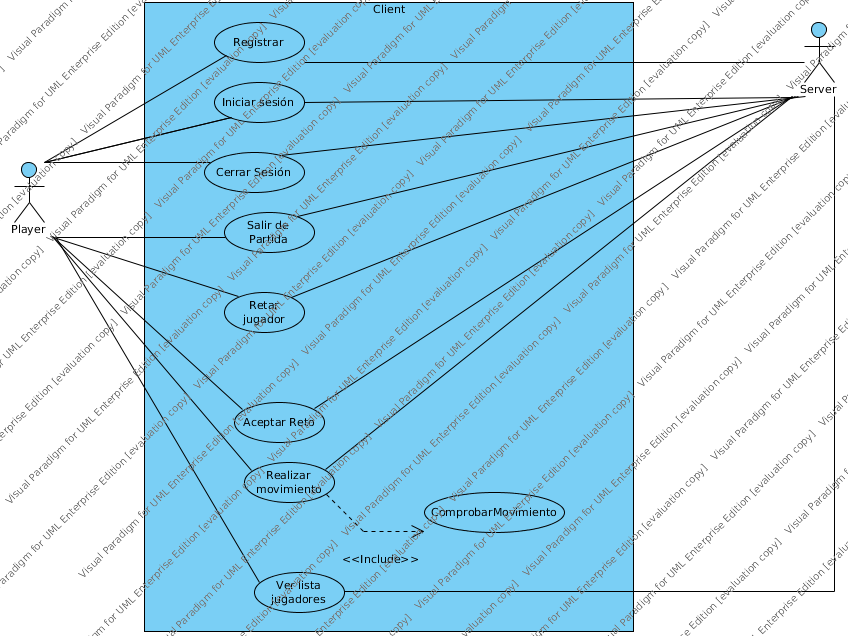
\includegraphics[scale=0.6]{img/cdu_Cliente.png}
 \caption{Diagrama de casos de uso del cliente}
 \label{cdu_cliente}
 \end{figure}
\clearpage
\subsection{Diagrama de casos de uso del servidor}
 \begin{figure}[h]
 \centering
 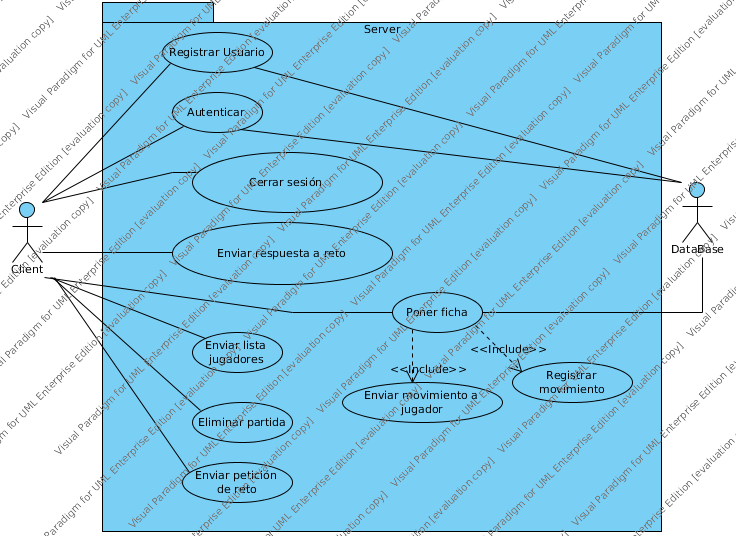
\includegraphics[scale=0.7]{img/cdu_Servidor.png}
 \caption{Diagrama de casos de uso del servidor}
 \label{cdu_servidor}
 \end{figure}

\clearpage

\section{Diagramas de clases}
\subsection{Diagrama de clases del cliente}
\begin{landscape}
 \begin{figure}[h]
 \centering
 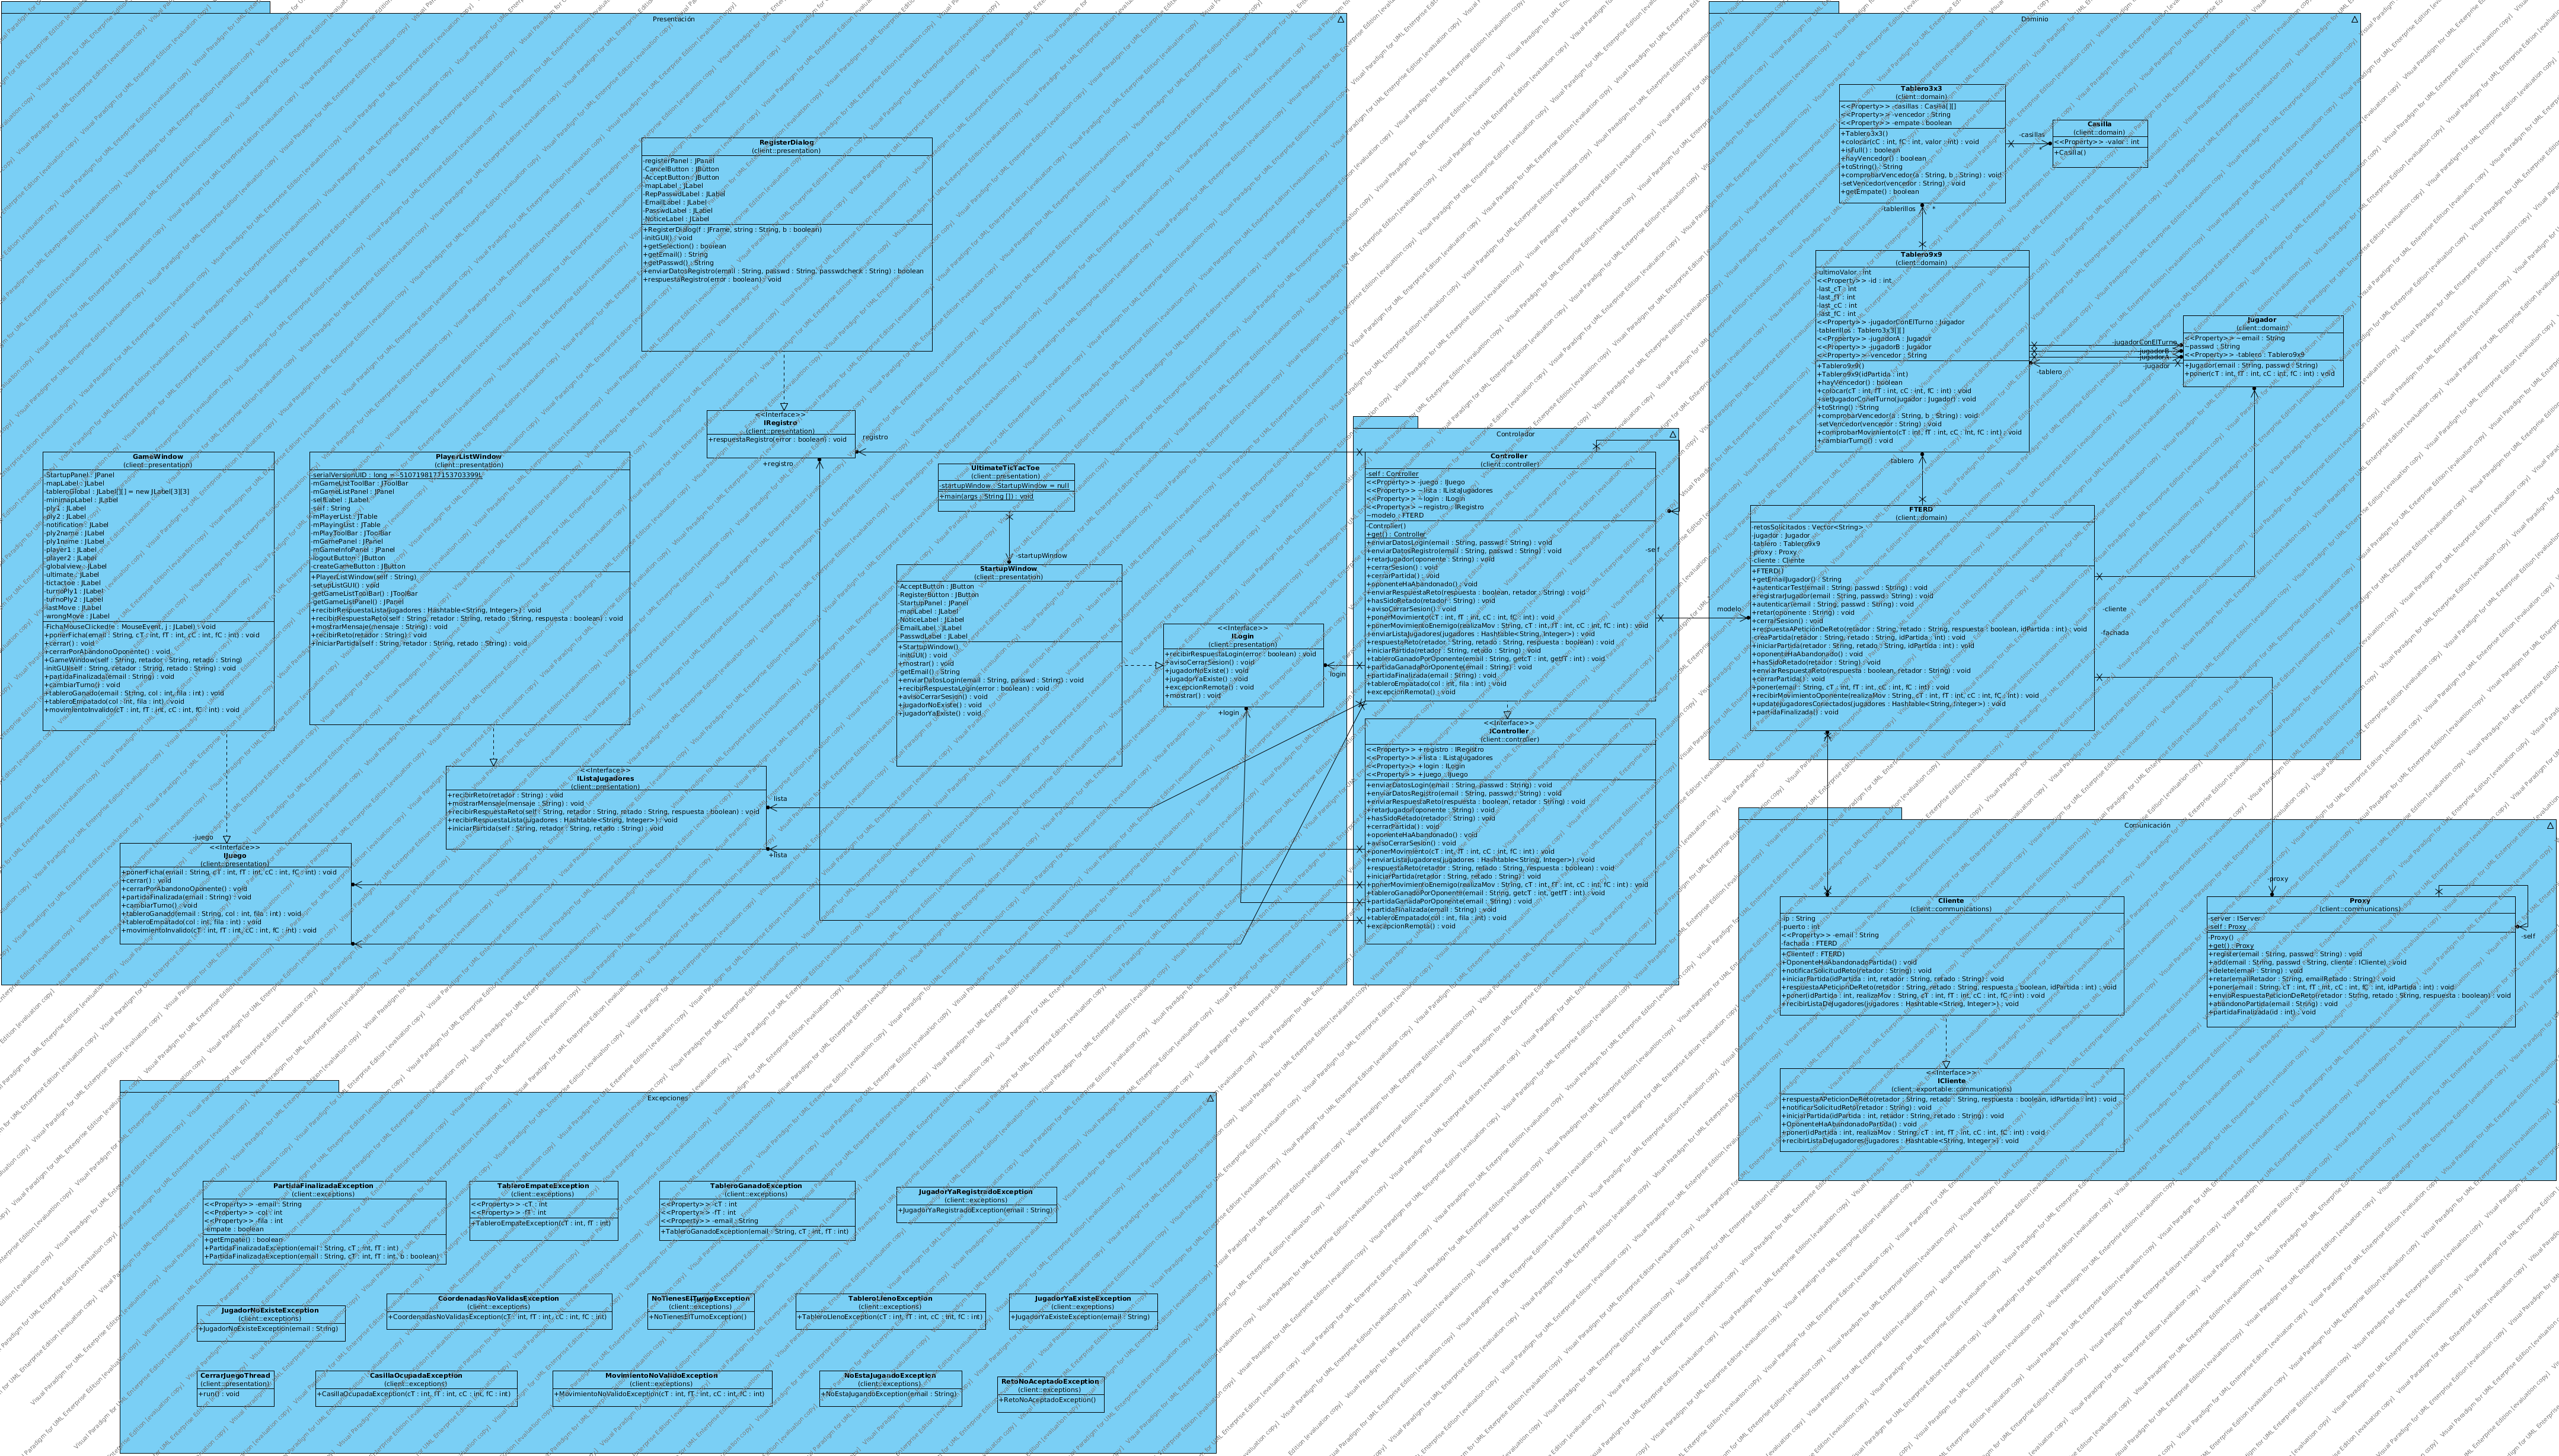
\includegraphics[scale=0.2]{img/ddc_Cliente.png}
 \caption{Diagrama de clases del cliente}
 \label{ddc_cliente}
 \end{figure}
\end{landscape}

\subsection{Diagrama de clases del servidor}
 \begin{figure}[h]
 \centering
 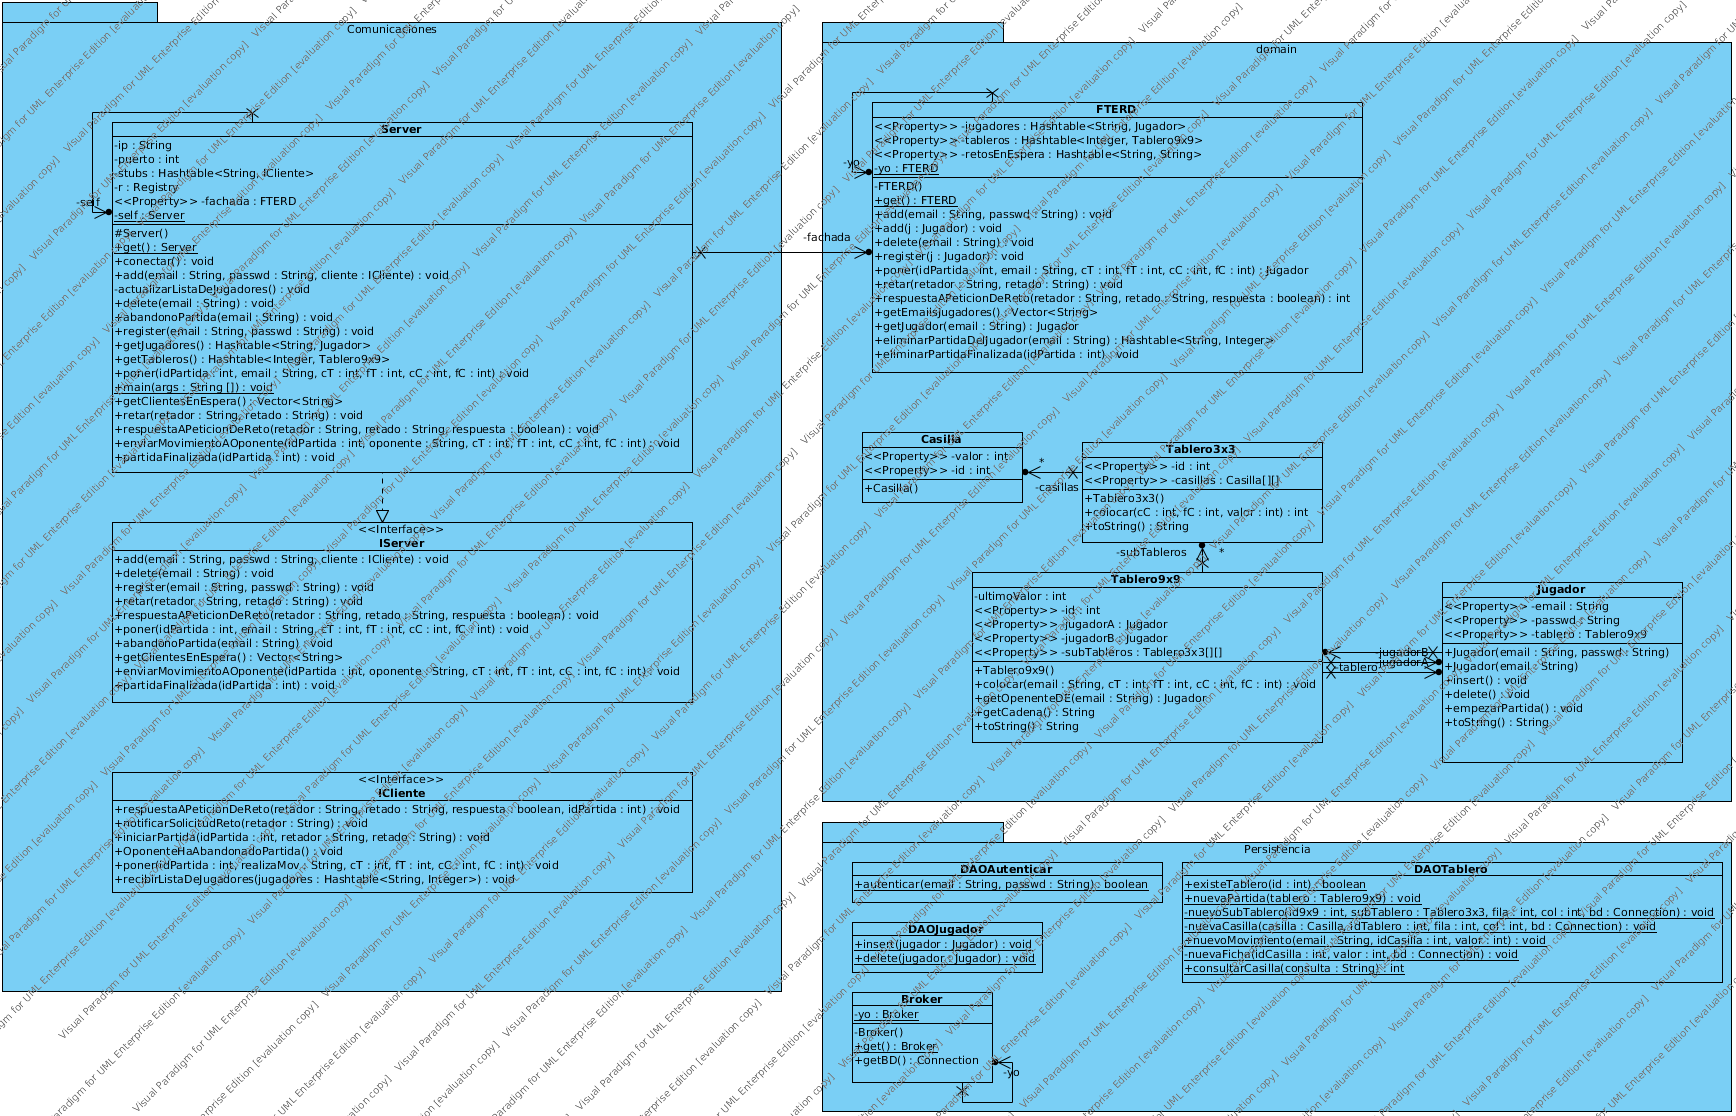
\includegraphics[scale=0.3]{img/ddc_Servidor.png}
 \caption{Diagrama de clases del servidor}
 \label{ddc_servidor}
 \end{figure}


\clearpage

\section{Diagramas de secuencia}
\subsection{Diagramas de secuencia del cliente}
\subsubsection{Autenticar}
 \begin{figure}[h]
 \centering
 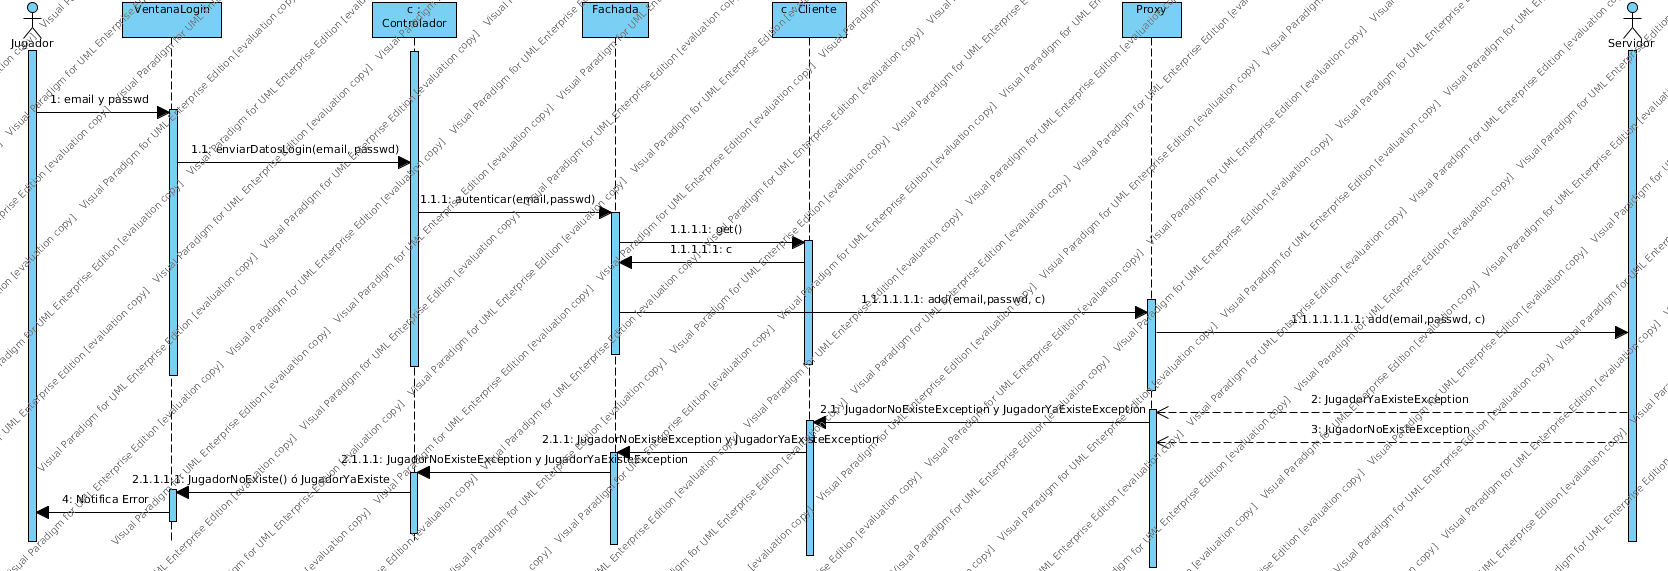
\includegraphics[scale=0.3]{img/ds_autenticar.png}
 \end{figure}
\subsubsection{Cerrar sesión oponente}
 \begin{figure}[h]
 \centering
 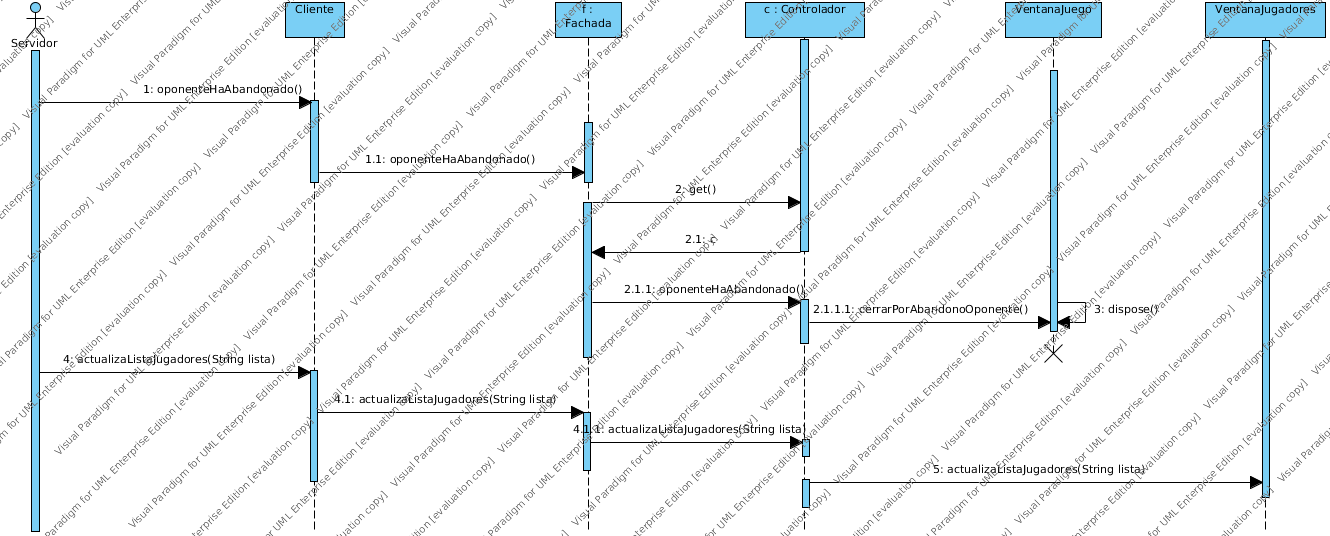
\includegraphics[scale=0.4]{img/ds_CerrarSesionOponenteCliente.png}
 \end{figure}
 \clearpage
\subsubsection{Enviar reto}
 \begin{figure}[h]
 \centering
 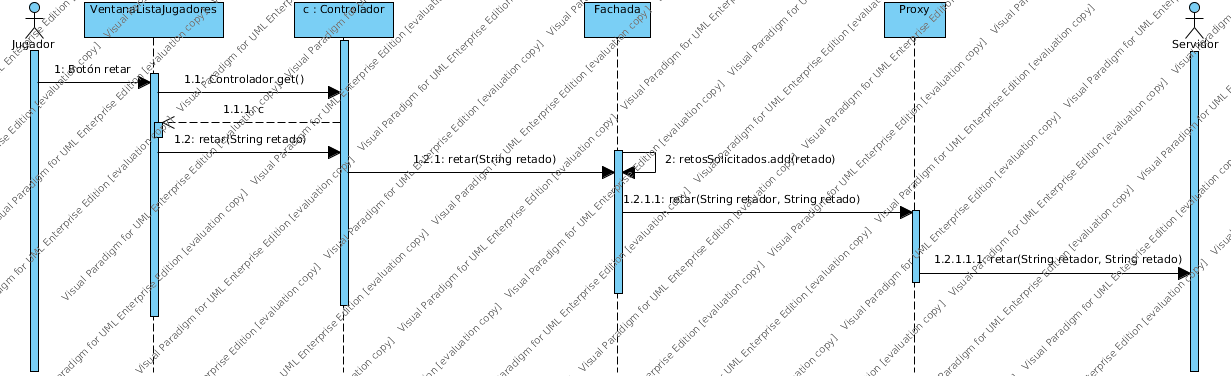
\includegraphics[scale=0.4]{img/ds_EnviarRetoCliente.png}
 \end{figure}
\subsubsection{Enviar respuesta reto}
 \begin{figure}[h]
 \centering
 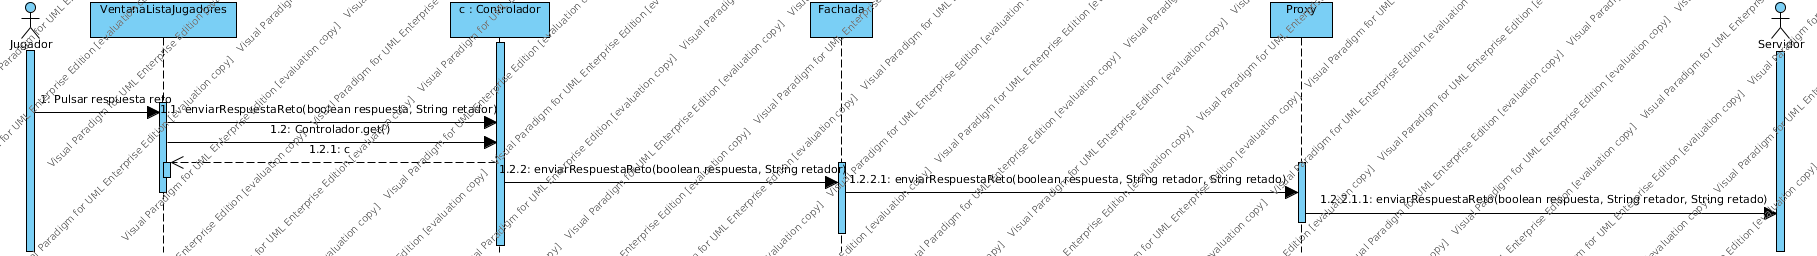
\includegraphics[scale=0.3]{img/ds_EnviarRespuestaRetoCliente.png}
 \end{figure}
 \clearpage
\subsubsection{Realizar movimiento}
 \begin{figure}[h]
 \centering
 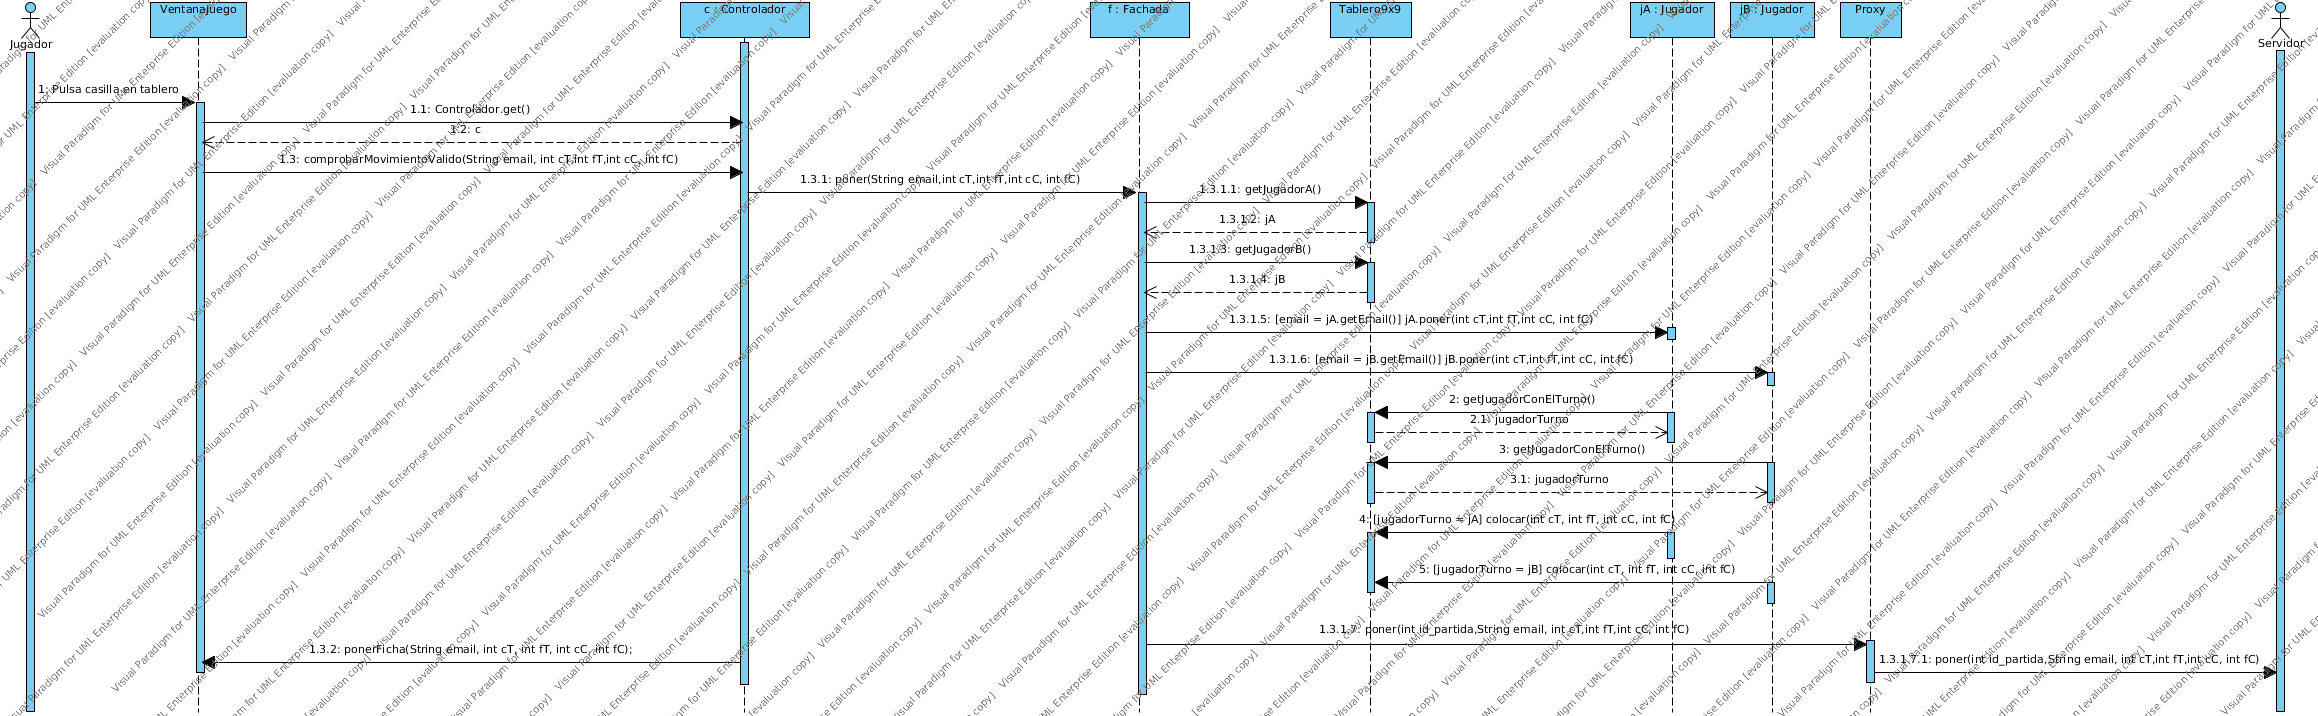
\includegraphics[scale=0.25]{img/ds_RealizarMovimientoCliente.png}
 \end{figure}
\subsubsection{Recibir movimiento}
 \begin{figure}[h]
 \centering
 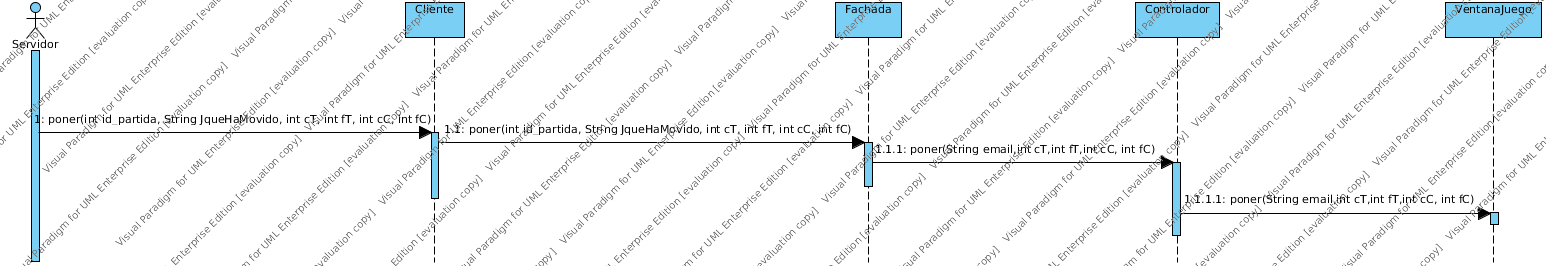
\includegraphics[scale=0.35]{img/ds_RecibirMovimientoCliente.png}
 \end{figure}
 \clearpage
\subsection{Diagramas de secuencia del servidor}
\subsubsection{Cerrar sesión}
 \begin{figure}[h]
 \centering
 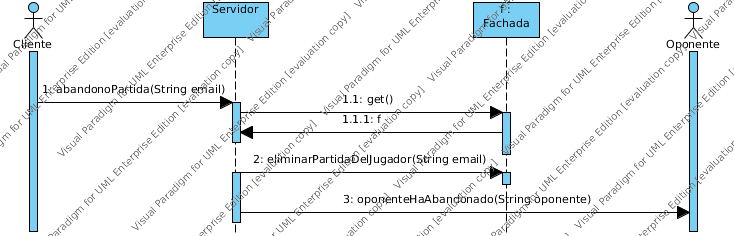
\includegraphics[scale=0.7]{img/ds_CerrarSesionServidor.png}
 \end{figure}
  \subsubsection{Enviar reto}
 \begin{figure}[h]
 \centering
 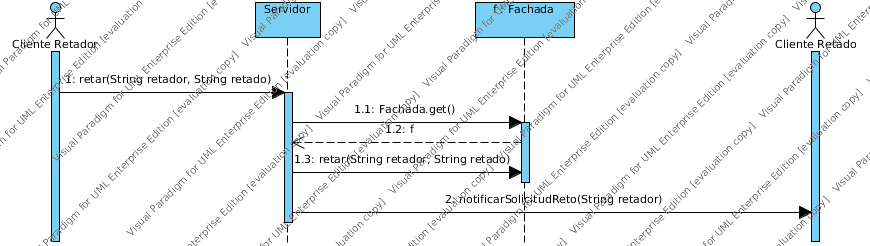
\includegraphics[scale=0.7]{img/ds_EnviarRetoServidor.png}
 \end{figure}
 \clearpage
 \subsubsection{Enviar respuesta reto}
 \begin{landscape}
 \begin{figure}[h]
 \centering
 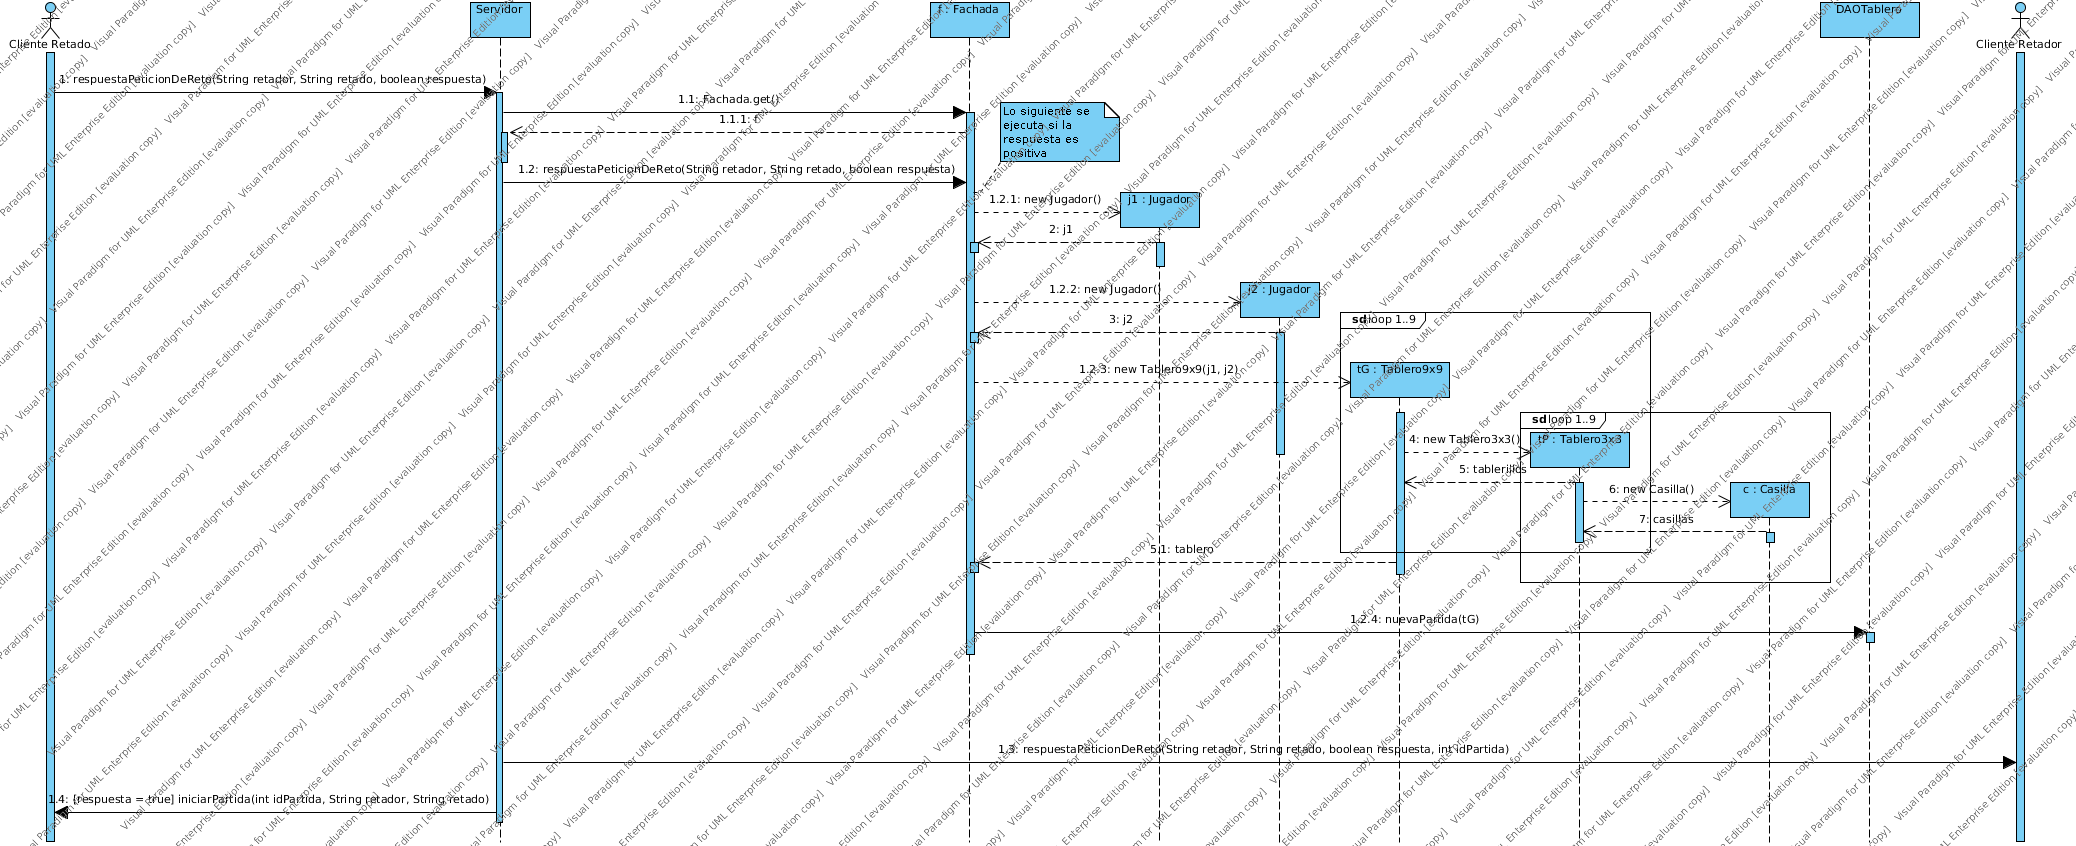
\includegraphics[scale=0.4]{img/ds_EnviarRespuestaRetoServidor.png}
 \end{figure}
  \end{landscape}
 \clearpage
\subsubsection{Realizar movimiento}
\begin{landscape}
 \begin{figure}[h]
 \centering
 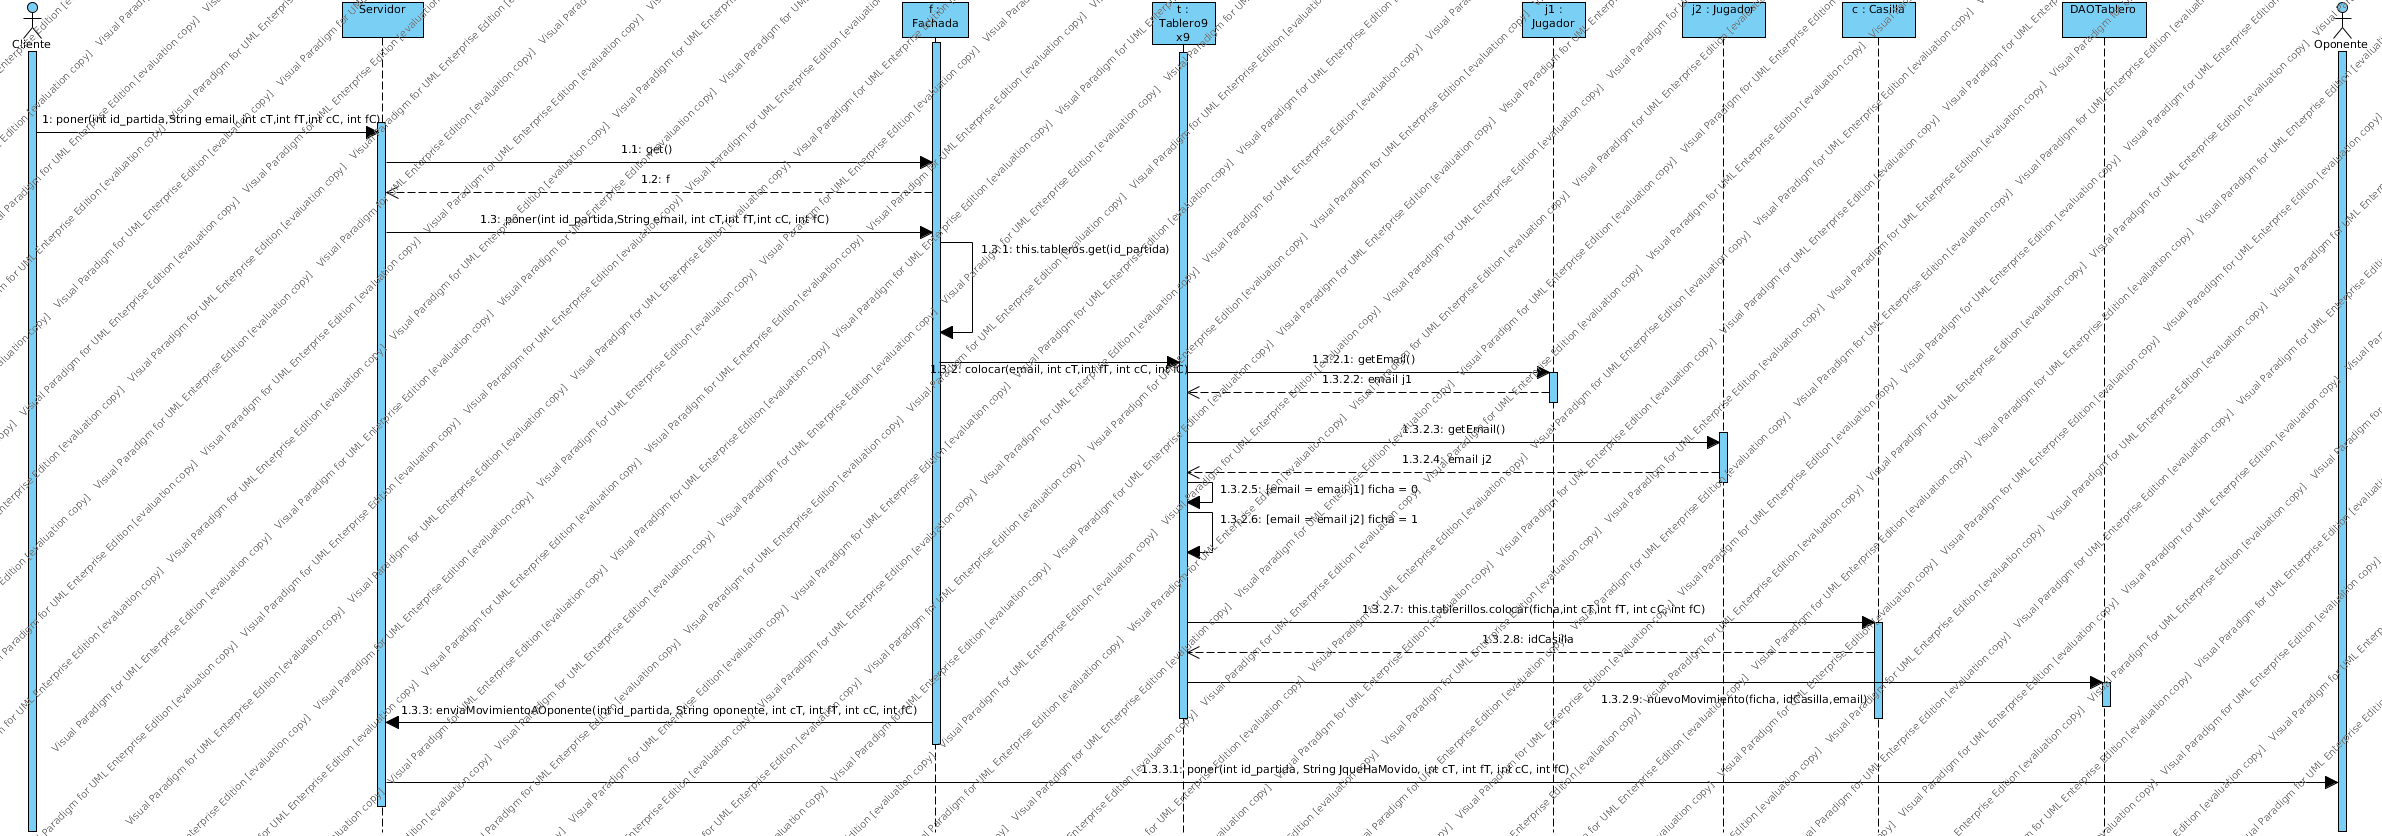
\includegraphics[scale=0.4]{img/ds_RealizarMovimientoServidor.png}
 \end{figure}
 \end{landscape}
 \clearpage


\clearpage

\section{Máquinas de estado}
\subsection{Máquinas de estado del cliente}
\subsubsection{Iniciar sesión}
 \begin{figure}[h]
 \centering
 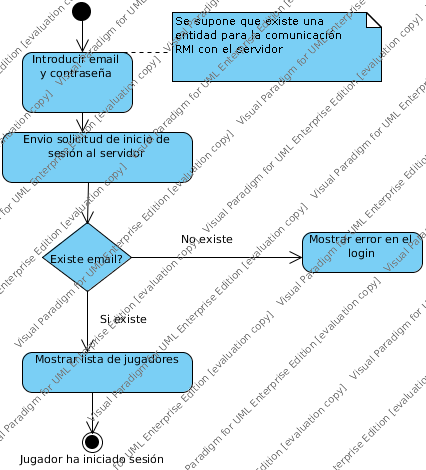
\includegraphics[scale=0.5]{img/ms_IniciarSesionCliente.png}
 \end{figure}
\subsubsection{Cerrar sesión}
 \begin{figure}[h]
 \centering
 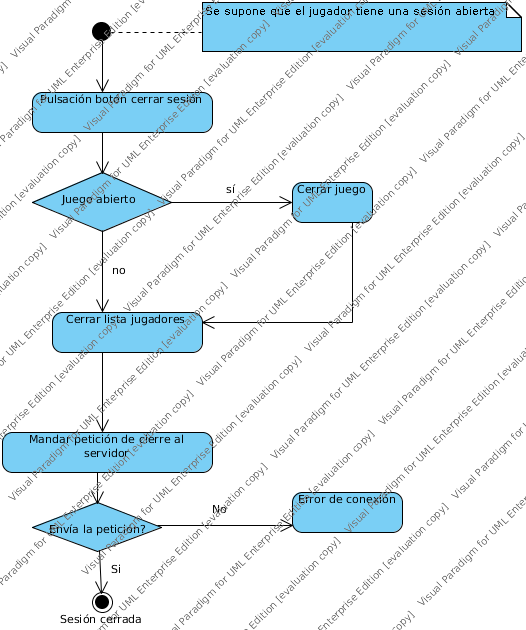
\includegraphics[scale=0.5]{img/ms_CerrarSesionCliente.png}
 \end{figure}
\subsubsection{Retar jugador}
 \begin{figure}[h]
 \centering
 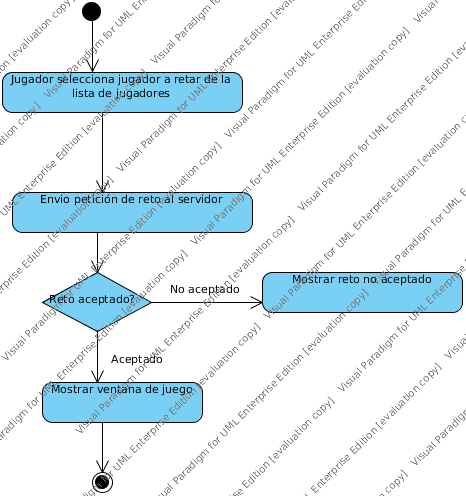
\includegraphics[scale=0.5]{img/ms_RetarJugadorCliente.png}
 \end{figure}
\subsubsection{Aceptar reto}
 \begin{figure}[h]
 \centering
 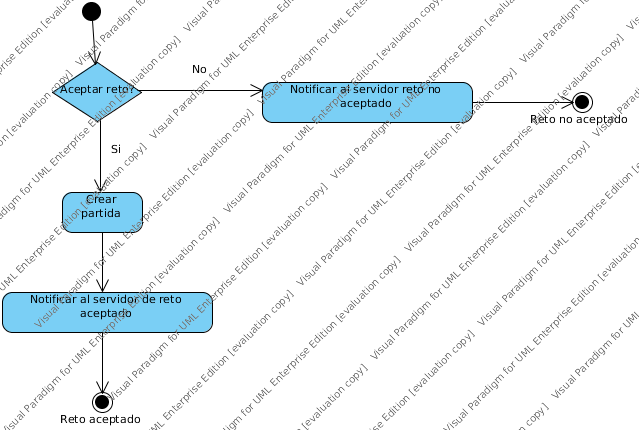
\includegraphics[scale=0.5]{img/ms_aceptarRetoCliente.png}
 \end{figure}
 \clearpage
\subsubsection{Realizar movimiento}
 \begin{figure}[h]
 \centering
 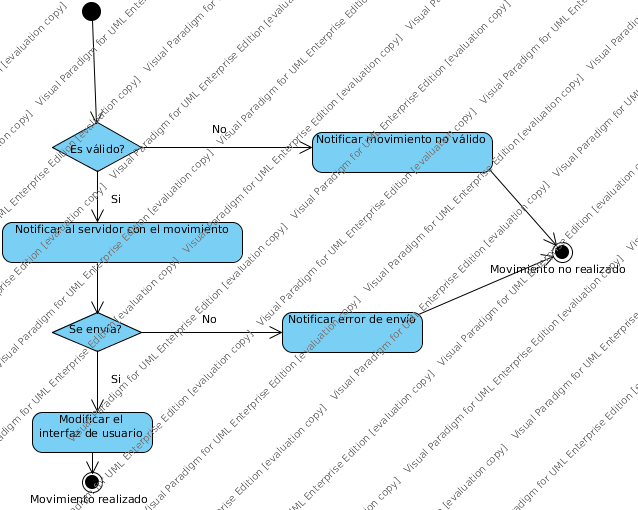
\includegraphics[scale=0.5]{img/ms_RealizarMovimientoCliente.png}
 \end{figure}
\subsubsection{Salir de partida}
 \begin{figure}[h]
 \centering
 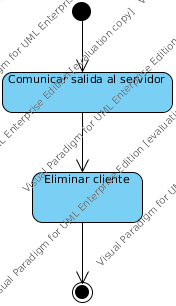
\includegraphics[scale=0.5]{img/ms_SalirPartidaCliente.png}
 \end{figure}
 \clearpage
\subsection{Máquinas de estado del servidor}
\subsubsection{Autenticar}
 \begin{figure}[h]
 \centering
 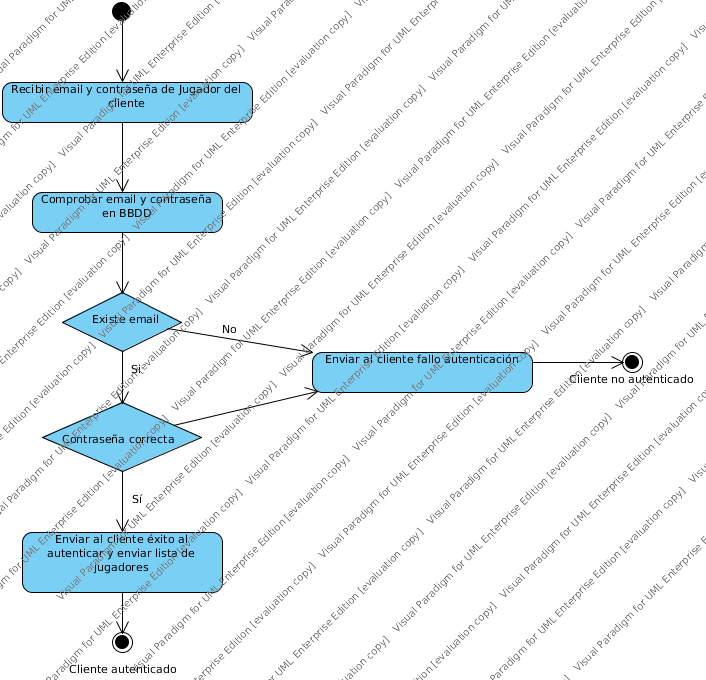
\includegraphics[scale=0.5]{img/ms_AutenticarServidor.png}
 \end{figure}
\subsubsection{Borrar partida}
 \begin{figure}[h]
 \centering
 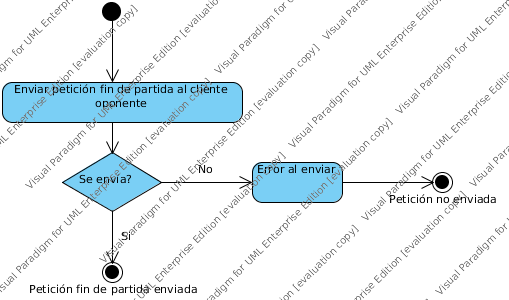
\includegraphics[scale=0.5]{img/ms_BorrarPartidaServidor.png}
 \end{figure}
 \clearpage
\subsubsection{Cerrar sesión}
 \begin{figure}[h]
 \centering
 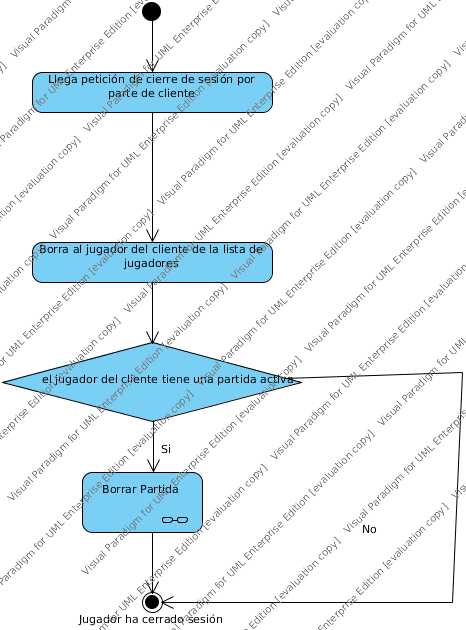
\includegraphics[scale=0.5]{img/ms_CerrarSesionServidor.png}
 \end{figure}
\subsubsection{Poner ficha}
 \begin{figure}[h]
 \centering
 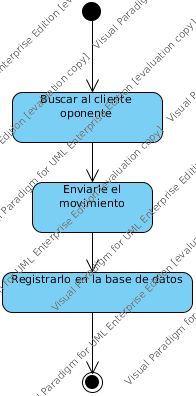
\includegraphics[scale=0.5]{img/ms_PonerFichaServidor.png}
 \end{figure}
 \clearpage
\subsubsection{Registrar usuario}
 \begin{figure}[h]
 \centering
 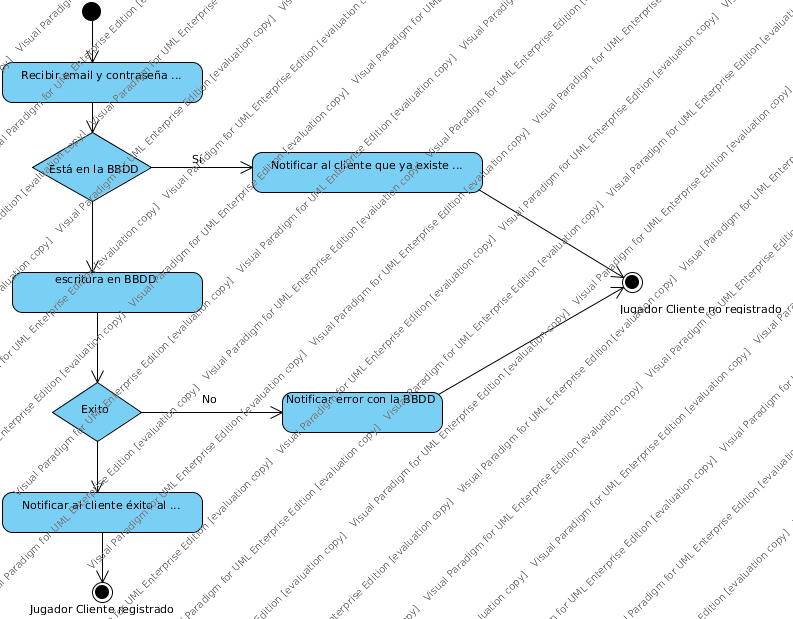
\includegraphics[scale=0.5]{img/ms_RegistrarUsuarioServidor.png}
 \end{figure}
\subsubsection{Retar jugador}
 \begin{figure}[h]
 \centering
 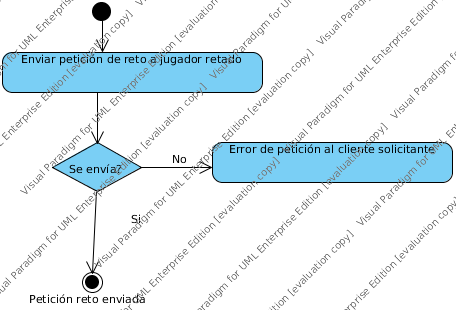
\includegraphics[scale=0.5]{img/ms_RetarJugadorServidor.png}
 \end{figure}
 \clearpage
\subsubsection{Respuesta a reto}
 \begin{figure}[h]
 \centering
 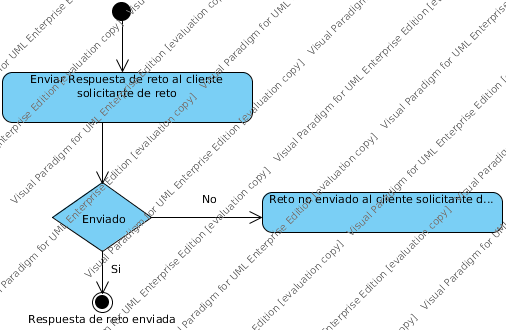
\includegraphics[scale=0.5]{img/ms_RespuestaRetoServidor.png}
 \end{figure}
 
\clearpage

\section{Pruebas de los casos de uso}

\subsection{Pruebas para la aplicación web}

Los test de la aplicación web han sido llevado a cabo mediante el testbed \emph{Selenium}. Las pruebas que han podido ser cubiertas y reproducibles han sido:

\begin{itemize}
\item Pruebas relacionadas con el login, posibles causas de error y de éxito.
\item Pruebas relacionadas con el registro, posibles causas de error y de éxito.
\item Pruebas relacionadas con el cierre de sesión, posibles causas de error y de éxito.
\end{itemize}

Para poder realizar estas pruebas ha sido necesario introducir una clase \emph{Broker} para la comunicación con la base de datos y una clase auxiliar que contiene las operaciones de borrado de esta base de datos.

Las pruebas relacionadas con la lógica de dominio por parte del cliente quedan cubiertas con las pruebas que se realizaron para el cliente web, ya que el código se ha cogido tal cual de esa implementación.

Se ha intentado realizar una prueba respecto de la jugabilidad, pero al no ser reproducible, se ha descartado. Estas pruebas han sido llevadas a cabo de forma manual con mucha dedicación y esfuerzo, probando las múltiples posibilidades para poder llevar la cobertura al máximo posible.

Las pruebas se encuentran en el paquete \emph{test.terd.web}.

\clearpage

\end{document}
